\documentclass{article}
\usepackage{amsmath}
\usepackage{amssymb}
\usepackage{tikz}
\usetikzlibrary{arrows.meta}

\begin{document}

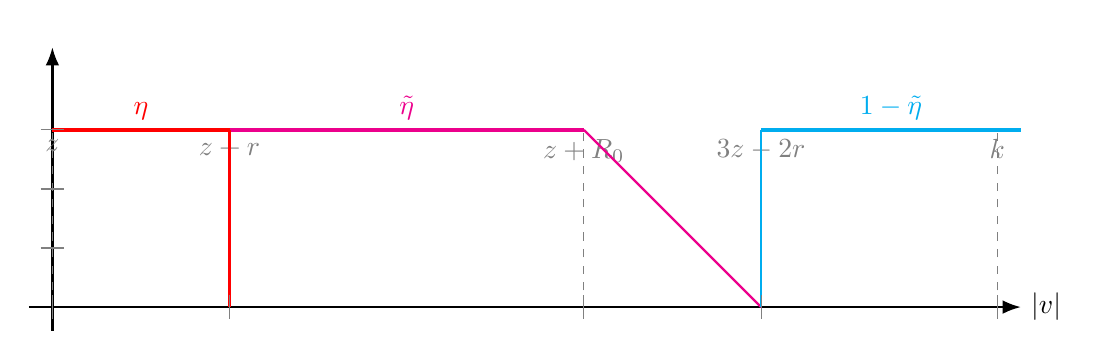
\begin{tikzpicture}[scale=1.5]

    % Axes
    \draw[-Latex, thick] (-0.2, 0) -- (8.2, 0) node[right] {$|v|$};
    \draw[-Latex, thick] (0, -0.2) -- (0, 2.2) node[above] {};

    % Horizontal lines
    \draw[red, very thick] (0, 1.5) -- (1.5, 1.5);
    \draw[magenta, very thick] (1.5, 1.5) -- (4.5, 1.5);
    \draw[cyan, very thick] (6, 1.5) -- (8.2, 1.5);

    % Vertical line indicating cutoff
    \draw[red, very thick] (1.5, 0) -- (1.5, 1.5);

    % Dashed vertical lines for labels
    \foreach \x/\label in {0/z, 1.5/z+r, 4.5/z+R_0, 6/3z-2r, 8/k}
        \draw[dashed, gray] (\x, 0) -- (\x, 1.5) node[below] {$\label$};

    % Labels for horizontal segments
    \node[red, above] at (0.75, 1.5) {$\eta$};
    \node[magenta, above] at (3, 1.5) {$\tilde{\eta}$};
    \node[cyan, above] at (7.1, 1.5) {$1-\tilde{\eta}$};

    % Slanted lines
    \draw[red, thick] (1.5, 1.5) -- (1.5, 0);
    \draw[magenta, thick] (4.5, 1.5) -- (6, 0);
    \draw[cyan, thick] (6, 0) -- (6, 1.5);

    % Ticks on the vertical axis
    \foreach \y in {0.5, 1, 1.5}
        \draw[gray] (-0.1, \y) -- (0.1, \y);

    % Tick marks on the horizontal axis
    \foreach \x in {0, 1.5, 4.5, 6, 8}
        \draw[gray] (\x, -0.1) -- (\x, 0.1);

\end{tikzpicture}

\end{document}